\documentclass[11pt,aspectratio=169]{beamer}
\usepackage[T1]{fontenc}
\usepackage{lmodern}
\usepackage{amsmath,amssymb,mathtools}
\usepackage{booktabs,tabularx,array}
\usepackage{pgfplots}
\pgfplotsset{compat=1.17}
\setbeamertemplate{navigation symbols}{}
\setbeamertemplate{itemize items}[circle]
\setbeamertemplate{footline}[frame number]
\setbeamerfont{framesubtitle}{size=\small}
\linespread{1.08}
\definecolor{plotblue}{RGB}{47,74,135}
\newcolumntype{Y}{>{\raggedright\arraybackslash}X}
\title{JMP progress, September 17--30, 2026}
\author{Tommaso De Santo}
\date{September 30, 2026}
\hypersetup{pdftitle={JMP progress, September 17--30, 2026},pdfauthor={Tommaso De Santo}}
% Separate adviser progress deck. Main source latex/JMP_slides/JMP_slides.tex is read-only.
% Exactly ten frames, no overlays or separate title/section/appendix pages.
% Relative source paths below are in Fertility_Spring26. See source_map.md for full paths.
\begin{document}

% 1: Reviewed changes to model specification and empirical inputs.
\begin{frame}{Model review and revisions}
\framesubtitle{JMP progress, September 17--30, 2026 \qquad | \qquad Tommaso De Santo}
\small
I reviewed preferences, household finance, demographic accounting, and the empirical calibration inputs.
\medskip
\begin{itemize}\setlength\itemsep{7pt}
 \item Replaced the minimum-housing requirement with a first-child increase in the housing expenditure share.
 \item Allowed diminishing benefits from children at home, distinguishing them from children ever born.
 \item Separated children leaving home from adult household entry, and tied entrant assets to estates.
 \item Rebuilt the first-birth housing evidence and recalibrated the revised model.
\end{itemize}
\end{frame}

% 2: Household choices and lifecycle risks in the retained model.
\begin{frame}{Household decisions}
\small
Overlapping generations of households differ in age, earnings, wealth, housing tenure, and family size.
\medskip
\begin{itemize}\setlength\itemsep{7pt}
 \item During fertile ages, households choose whether to attempt a birth; success becomes less likely with age.
 \item They choose consumption, saving, housing size, and whether to rent or own; renters pay rent, while owners make a down payment and face selling costs.
 \item Persistent earnings risk and borrowing limits shape saving; a first-birth fixed cost and taste shocks shape fertility.
 \item Households retire, face mortality risk, and value bequests.
\end{itemize}
\vfill
The interaction of housing costs and available wealth affects both birth timing and tenure choice.
\end{frame}

% 3: Household preference equations and definitions from the verified reference.
\begin{frame}{Children and housing demand}
\small
Households consume nonhousing goods $c$ and housing services $s$, and derive
utility from the $m$ children living at home:
\[
 u(c,s,m)=\frac{\left[\dfrac{A(m)c^{\alpha(m)}s^{1-\alpha(m)}}{e(m)}\right]^{1-\sigma}}{1-\sigma}
 +\psi m^{1-\gamma}.
\]
The equivalence scale $e(m)$ captures the consumption cost of a larger family;
$\sigma$ governs risk aversion. The benefit from children is zero at $m=0$,
with $\psi$ setting its level and $\gamma$ its curvature.
\par\medskip
Having children also raises the share of expenditure devoted to housing:
\[
 \alpha(m)=\alpha_0-\Delta\alpha\,\mathbf 1\{m>0\}.
\]
$\alpha_0$ is the childless consumption share. The first child raises the
housing share by $\Delta\alpha$; additional children leave that share unchanged.
\par\medskip
For given spending and family size, $A(m)$ offsets the utility effect of the
share change at a fixed reference rent.
\end{frame}

% 4: Demographic transitions and market/fiscal closure.
\begin{frame}{Demographic and market equilibrium}
\small
Children leaving home and new adult households entering the economy are separate transitions.
\medskip
\begin{itemize}\setlength\itemsep{5pt}
 \item Children leave dependency independently; adult entry follows earlier births with a lag.
 \item Positive estates finance fixed positive entrant assets; any remainder leaves the economy.
 \item The house price clears aggregate housing demand against housing supply.
 \item Equal retiree pensions are financed by a balanced payroll tax.
\end{itemize}
\vfill
A stationary equilibrium has constant prices, allocations, and cohort structure, with demographic reproduction and market clearing.
\end{frame}

% 5: PSID event-study estimates; raw coefficients and pointwise intervals.
\begin{frame}{Housing around the first birth}
\small
I rebuilt the PSID event study using interview dates and household status before the first birth.
\begin{center}
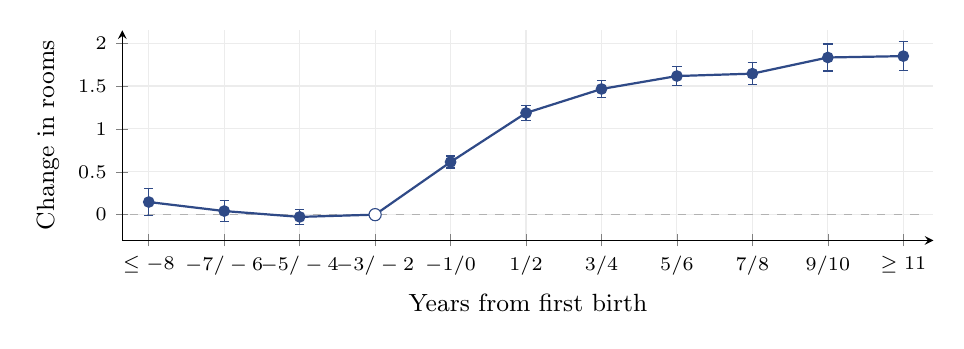
\begin{tikzpicture}
\begin{axis}[
 width=0.98\textwidth,height=4.25cm,
 xmin=-9.2,xmax=12.3,ymin=-0.3,ymax=2.15,
 xlabel={Years from first birth},ylabel={Change in rooms},
 xtick={-8.5,-6.5,-4.5,-2.5,-.5,1.5,3.5,5.5,7.5,9.5,11.5},
 xticklabels={$\leq-8$,$-7/-6$,$-5/-4$,$-3/-2$,$-1/0$,$1/2$,$3/4$,$5/6$,$7/8$,$9/10$,$\geq11$},
 tick label style={font=\scriptsize},label style={font=\small},
 axis lines=left,grid=major,grid style={gray!15},
 ytick={0,.5,1,1.5,2},
]
\addplot[gray!60,dashed] coordinates {(-9,0) (12,0)};
\addplot[plotblue,thick,mark=*,mark size=1.7pt,error bars/.cd,y dir=both,y explicit]
 table[x=x,y=y,y error=err,row sep=\\]{
 x y err\\
 -8.5 .147277343 .158189222\\
 -6.5 .042068289 .119348387\\
 -4.5 -.026169280 .087417230\\
 -2.5 0 0\\
 -.5 .613924680 .070093112\\
 1.5 1.185961330 .083049105\\
 3.5 1.465293280 .098529943\\
 5.5 1.616432695 .111654038\\
 7.5 1.644179690 .127752165\\
 9.5 1.832730146 .157289669\\
 11.5 1.848654304 .168139494\\
 };
\addplot[plotblue,only marks,mark=*,mark size=2.2pt,mark options={fill=white}] coordinates {(-2.5,0)};
\end{axis}
\end{tikzpicture}
\end{center}
\vspace{-0.8em}
At years 3--4, rooms rise by \textbf{1.465} (SE 0.050), ownership by
\textbf{26.886 pp}, and recent moving falls by \textbf{21.147 pp}.
\par\medskip
\footnotesize Reference person or spouse before birth. Baseline: years $-3/-2$;
person and year effects; survey weights; 95\% pointwise intervals.
\end{frame}

% 6: Adopted national inputs and empirical counterparts; September 28 reference.
\begin{frame}{Calibration strategy and inputs}
\small
I recalibrated the 2007 stationary economy after revising the empirical inputs.
\medskip
\begin{center}
\begin{tabular}{lll}
\toprule
Input & Value & Measurement \\
\midrule
Mean occupied rooms & 5.729 & AHS 2007 \\
Pension / working-household earnings & 0.229 & CPS ASEC, income 2007 \\
Annual child-directed estates / wealth & 0.729\% & SCF 2007 mortality proxy \\
Annual depreciation / property tax & 1.416\% / 1.060\% & National housing inputs \\
\bottomrule
\end{tabular}
\end{center}
\medskip
\begin{itemize}\setlength\itemsep{4pt}
 \item The calibration matches fertility, wealth, housing size, and tenure; completed fertility is normalized to 2.1.
 \item The first-birth housing comparison still uses a model proxy for the empirical event study.
\end{itemize}
\vfill
A period is four years. Each dependent child leaves with probability $2/9$;
adult entry is split equally between 16 and 20 years after birth.
\end{frame}

% 7: Full 14-row 2007 stationary reference fit; ten scored moments plus normalization.
\begin{frame}{2007 stationary calibration}
\centering
\fontsize{9}{10.7}\selectfont
{\centering\renewcommand{\arraystretch}{0.95}\setlength{\tabcolsep}{10pt}
\begin{tabular}{lrr}
\toprule
Moment & Target & Model \\
\midrule
Completed fertility (normalization) & 2.100 & 2.100 \\
Childlessness, ages 40--44 (\%) & 19.828 & 20.106 \\
Exactly one child among mothers, ages 40--44 (\%) & 21.366 & 20.942 \\
Mean first-birth age (years) & 25.976 & 25.933 \\
First births at age 30+ (\%)$^\dagger$ & 24.928 & 22.365 \\
Wealth / earnings & 6.927 & 6.326 \\
Annual child-directed bequest flow / wealth (\%) & 0.729 & 0.706 \\
Older wealth/income p90/p50$^\dagger$ & 3.516 & 3.069 \\
Mean occupied rooms & 5.729 & 5.848 \\
Ownership, ages 30--55 (\%) & 67.626 & 65.482 \\
First-birth rooms difference & 1.465 & 1.622 \\
Family rooms difference$^\dagger$ & 0.385 & 0.353 \\
Recent-parent ownership difference (pp) & 12.761 & 11.955 \\
\textbf{Children per woman at age 25, capped at three} & \textbf{0.810} & \textbf{0.535} \\
\bottomrule
\end{tabular}
\par}
\vspace{0.4em}
\footnotesize $^\dagger$Untargeted validation. Ten scored moments and a separate fertility normalization.
\end{frame}

% 8: Ten free reference coordinates and normalized child benefit.
\begin{frame}{Calibrated parameters}
\small
The reference estimates ten free parameters and separately normalizes the child-benefit level.
\medskip
\fontsize{9}{10.7}\selectfont
\begin{center}
{\setlength{\tabcolsep}{10pt}
\begin{tabular}{llr}
\toprule
Parameter & Economic interpretation & Value \\
\midrule
$H_0$ & Housing supply scale & 6.294 \\
$\beta$ & Annual discount factor & 0.963 \\
$\chi$ & Owner housing-service premium & 1.094 \\
$F_1$ & First-birth fixed utility cost & 0.621 \\
$\kappa_1$ & First-birth taste dispersion & 0.176 \\
$\kappa_+$ & Later-birth taste dispersion & 0.332 \\
$\theta_0$ & Bequest weight & 0.125 \\
$\Delta\alpha$ & First-child housing-share loading & 0.135 \\
$\gamma$ & Child-benefit curvature & 0.061 \\
$\kappa_T$ & Tenure-choice dispersion & 0.012 \\
$\psi$ & Child-benefit level (normalized) & 0.136 \\
\bottomrule
\end{tabular}
}
\end{center}
\vfill
\footnotesize Fixed inputs: $\sigma=2$; $\alpha_0=0.733$; annual interest 2\%; mortgage-financed share 80\%.
\end{frame}

% 9: Later experimental age-25 fertility comparisons; no adoption implied.
\begin{frame}{Fertility at young ages}
\small
Subsequent experimental calibrations, with completed fertility normalized to 2.1:
\medskip
\begin{center}
\begin{tabular}{lrrr}
\toprule
Age-25 moment & Data & \shortstack{One birth\\per period} & \shortstack{Two-birth\\option} \\
\midrule
Children per woman, capped at three & 0.810 & 0.530 & 0.606 \\
Mothers (\%) & 45.725 & 44.782 & 43.773 \\
Children per mother, capped at three & 1.770 & 1.185 & 1.385 \\
\bottomrule
\end{tabular}
\end{center}
\medskip
\begin{itemize}\setlength\itemsep{4pt}
 \item The share of mothers is close to the data; births among young mothers are too few.
 \item Allowing two births per period closes 27.1\% of the child-count gap, with worse fit elsewhere.
\end{itemize}
\vfill
The extension also adds a taste draw, so this comparison does not isolate birth spacing.
\end{frame}

% 10: Completed, experimental entrant-wealth calibration pilots; no adoption.
\begin{frame}{Credit and further calibration}
\small
I reviewed the borrowing rules and tested alternative initial-wealth distributions at a common 2\% annual real interest rate.
\medskip
\begin{center}
\begin{tabularx}{\textwidth}{Y r}
\toprule
Entrant wealth rule & \shortstack{Renter debt limit\\(mean annual earnings)} \\
\midrule
Empirical wealth/earnings ratios drawn independently of earnings & 0.25 \\
Zero entrant wealth & 0 \\
Nonnegative ratio distribution with the original mean & 0 \\
\bottomrule
\end{tabularx}
\end{center}
\medskip
\begin{itemize}\setlength\itemsep{5pt}
 \item The three pilot calibrations are complete; an entrant-wealth and credit specification has yet to be selected.
 \item The next step is to resolve that choice and assess the remaining young-fertility gap.
\end{itemize}
\vfill
The stationary solver was reorganized and accelerated to support calibration.
\end{frame}

\end{document}
